% CCAT 2026 (Fukuoka) camera-ready. IEEE conference format (IEEEtran.cls).
\documentclass[conference]{IEEEtran}
\IEEEoverridecommandlockouts

\usepackage{cite}
\usepackage{amsmath,amssymb,amsfonts}
\usepackage{graphicx}
\usepackage{textcomp}
\usepackage{xcolor}
\usepackage{booktabs}
\usepackage{multirow}
\usepackage{array}
\usepackage[hyphens]{url}
\Urlmuskip=0mu plus 1mu

\graphicspath{{figures/}}

\begin{document}

\title{A Comparative Study of CNN-Based, Transformer-Based, and Open-Vocabulary Detectors for Cargo Container and Scene Text Detection}

\author{%
\begin{tabular}{c@{\hspace{4em}}c}
\begin{tabular}{c}
Xin Yiing Loo \\
\textit{Transdisciplinary School}\\
\textit{University of Technology Sydney}\\
Sydney, Australia\\
XinYiing.Loo@student.uts.edu.au
\end{tabular}
&
\begin{tabular}{c}
Siyuan Yang \\
\textit{Transdisciplinary School}\\
\textit{University of Technology Sydney}\\
Sydney, Australia\\
Siyuan.Yang-1@student.uts.edu.au
\end{tabular}
\\[2.5em]
\begin{tabular}{c}
Xiaodan Dong\textsuperscript{*} \\
\textit{Transdisciplinary School}\\
\textit{University of Technology Sydney}\\
Sydney, Australia\\
Xiaodan.Dong@uts.edu.au\\
\textsuperscript{*}Corresponding author
\end{tabular}
&
\begin{tabular}{c}
Weidong Huang \\
\textit{Transdisciplinary School}\\
\textit{University of Technology Sydney}\\
Sydney, Australia\\
Weidong.Huang@uts.edu.au
\end{tabular}
\end{tabular}}

\maketitle

\begin{abstract}
Reading the printed identity code on a cargo container is a high-stakes step in port logistics, and it is difficult in practice because the code region is small, the capture conditions vary, and generic off-the-shelf text readers perform poorly on this domain. A natural question is whether open-vocabulary detection, which accepts category names as text prompts, can locate such targets without any domain-specific training and therefore remove the labelling step. This study examines that question by comparing three detection paradigms under a single evaluation protocol: a CNN-based detector (YOLOv8), a Transformer-based detector (RT-DETR), and an open-vocabulary vision-language detector (YOLO-World). The models are evaluated on a public single-class container-number dataset and on the ICDAR 2015 scene text dataset, both reported on a held-out test split, with COCO 2017 used as a reference check on the pipeline. The main finding is negative and reproducible. Zero-shot YOLO-World reaches only 0.0033 mAP50-95 on the container test split and 0.0018 on ICDAR 2015, and this failure persists across eight container and four scene-text prompt formulations, all below 0.10. Supervised training recovers the gap: fine-tuned YOLO-World reaches 0.9181 on the container data, and across the three trained models mAP50-95 is 0.90 to 0.92 on the container data and 0.42 to 0.45 on ICDAR 2015. RT-DETR is the most accurate detector on ICDAR 2015 at 0.4526 mAP50-95, but it runs about five times slower than YOLOv8 at inference. This study proposes no new architecture. Its contribution is reproducible empirical evidence that open-vocabulary pre-training, as implemented in YOLO-World, does not replace target-domain supervision for container and scene text detection, together with the prompt-sensitivity and inference-cost measurements needed to choose a detector for deployment.
\end{abstract}

\begin{IEEEkeywords}
object detection, container text detection, YOLOv8, RT-DETR, YOLO-World, open-vocabulary detection, scene text detection
\end{IEEEkeywords}

\section{Introduction}

Reading the printed identity code on a shipping container is a routine but high-stakes step in port and terminal operations. Each container carries an ISO 6346 code that is used to track it through the yard, and an error in reading this code propagates into the wrong record for the wrong container. Industry sources report that manual tracking can cost terminals a large share of productivity, and that even a one to two percent error rate across the many gate movements handled each day compounds into downstream problems \cite{allread2024maritime}. Automated reading is therefore attractive, but it must be reliable under operational conditions.

Operational imagery is not clean. Container codes are captured at gates and during handling, under changing light, at oblique and upward angles, on rusted and repainted surfaces, and in both horizontal and vertical ISO 6346 layouts \cite{scanbot2024iso6346}. Generic, off-the-shelf text readers do not handle this domain well. A recent study reports that a generic Tesseract pipeline reached only 0.41 percent text detection precision on container codes, while a system fine-tuned on task-specific data with manually drawn bounding boxes reached 99.40 percent detection precision and above 96 percent recognition accuracy \cite{santos2025container}. The practical implication is that current industrial systems still require manual annotation and per-domain training, which is a real cost.

This cost motivates the question studied here. Open-vocabulary detectors accept category names as text prompts and can be redirected to new targets without retraining, which suggests they might locate container text without any domain-specific labelling. This study asks whether that is the case, and answers it by comparing three detection paradigms under one protocol: a CNN-based detector, a Transformer-based detector, and an open-vocabulary detector. Most existing studies evaluate these paradigms on general benchmarks such as COCO, and there is limited evidence on how they behave on domain-specific industrial targets such as cargo container codes. The answer found here is negative. Zero-shot YOLO-World, the open-vocabulary detector evaluated here, almost completely fails on container and scene text, the failure is robust to how the prompt is worded, and target-domain fine-tuning is required to recover useful accuracy. This result is reported together with a mechanistic explanation, an inference-cost comparison, and a full configuration so that it can be reproduced.

The contribution of this study is threefold. First, the three paradigms are compared under a single evaluation protocol rather than across separately reported results. Second, YOLO-World is evaluated in zero-shot mode across several prompt formulations and after fine-tuning, which separates open-vocabulary pre-training from prompt wording and from target-domain supervision. Third, inference latency and memory are measured, so the comparison speaks to deployment and not only to accuracy.

The scope should be read narrowly. No new architecture, training strategy, or loss function is proposed. The container evaluation uses one public single-class dataset as an open proxy for the original industrial dataset, which is not publicly available, so that every reported number can be regenerated by a third party. The findings describe this setting and the prompts tested, and should not be generalised to industrial text detection as a whole.

\section{Related Work}

The YOLO family formulates detection as a one-stage problem in which a single network predicts bounding boxes and class probabilities directly from the input image, which avoids the region proposal stage and enables real-time inference \cite{redmon2016yolo,redmon2018yolov3}. YOLOv8 continues this development with an anchor-free detection head and multi-scale feature fusion through an FPN and PAN style neck \cite{yolov8}. These detectors are efficient and straightforward to train on custom datasets, but their label space is fixed at training time.

DETR treats detection as a direct set prediction problem and uses bipartite matching to assign predictions to ground-truth objects, which removes the need for anchors and non-maximum suppression \cite{carion2020detr}. Its original formulation trains slowly and performs relatively weakly on small objects, which later variants improved. RT-DETR adapts the paradigm to real-time detection while preserving the end-to-end formulation \cite{zhao2024rtdetr}.

Open-vocabulary detectors extend visual detection by using language as an additional source of task definition. Instead of predicting a fixed set of categories, they accept textual prompts or category names, so the same model can be redirected to different targets by changing the language input. GLIP aligns image regions with language prompts and shows strong zero-shot and few-shot transfer \cite{li2022glip}. ViLD distils semantic knowledge from a pretrained image-text model into a detector so that it can recognise categories absent from the detection annotations \cite{gu2022vild}. YOLO-World reformulates instance annotations as region-text pairs and uses a text contrastive head with text-guided feature aggregation, which retains prompt-based detection inside an efficient YOLO-style pipeline \cite{cheng2024yoloworld}. These models show that language supervision can improve adaptability, but they also introduce heavier dependencies. Few studies have examined their behaviour on cargo-domain industrial text, which is the gap this study addresses.

A separate line of work builds text-specialised detectors, including EAST \cite{zhou2017east}, TextSnake \cite{long2018textsnake}, DBNet \cite{liao2020dbnet}, and ABCNet \cite{liu2020abcnet}, which typically report polygon-based accuracy on scene text. They are not included here, because the aim is to compare general detection paradigms under one protocol and to test whether an open-vocabulary detector can locate the targets without domain supervision, not to reach the best scene text accuracy.

\section{Research Questions}

This study is guided by three questions.

\textbf{RQ1.} How do CNN-based and Transformer-based detectors compare on container text detection and on scene text detection?

\textbf{RQ2.} Can an open-vocabulary detector locate container and scene text targets in a zero-shot setting using textual prompts alone, and is the outcome sensitive to how the prompt is worded?

\textbf{RQ3.} How much does target-domain fine-tuning improve the open-vocabulary detector?

\section{Methodology}

\subsection{Model Selection}

Three models are selected, one from each paradigm, as shown in Fig.~\ref{fig:model_flowchart}. The term selected models refers to representative and practically testable models from each paradigm, rather than the single best-performing model reported in the literature. YOLOv8 is the CNN-based detector, RT-DETR is the Transformer-based detector, and YOLO-World is the open-vocabulary detector.

\begin{figure}[tb]
    \centering
    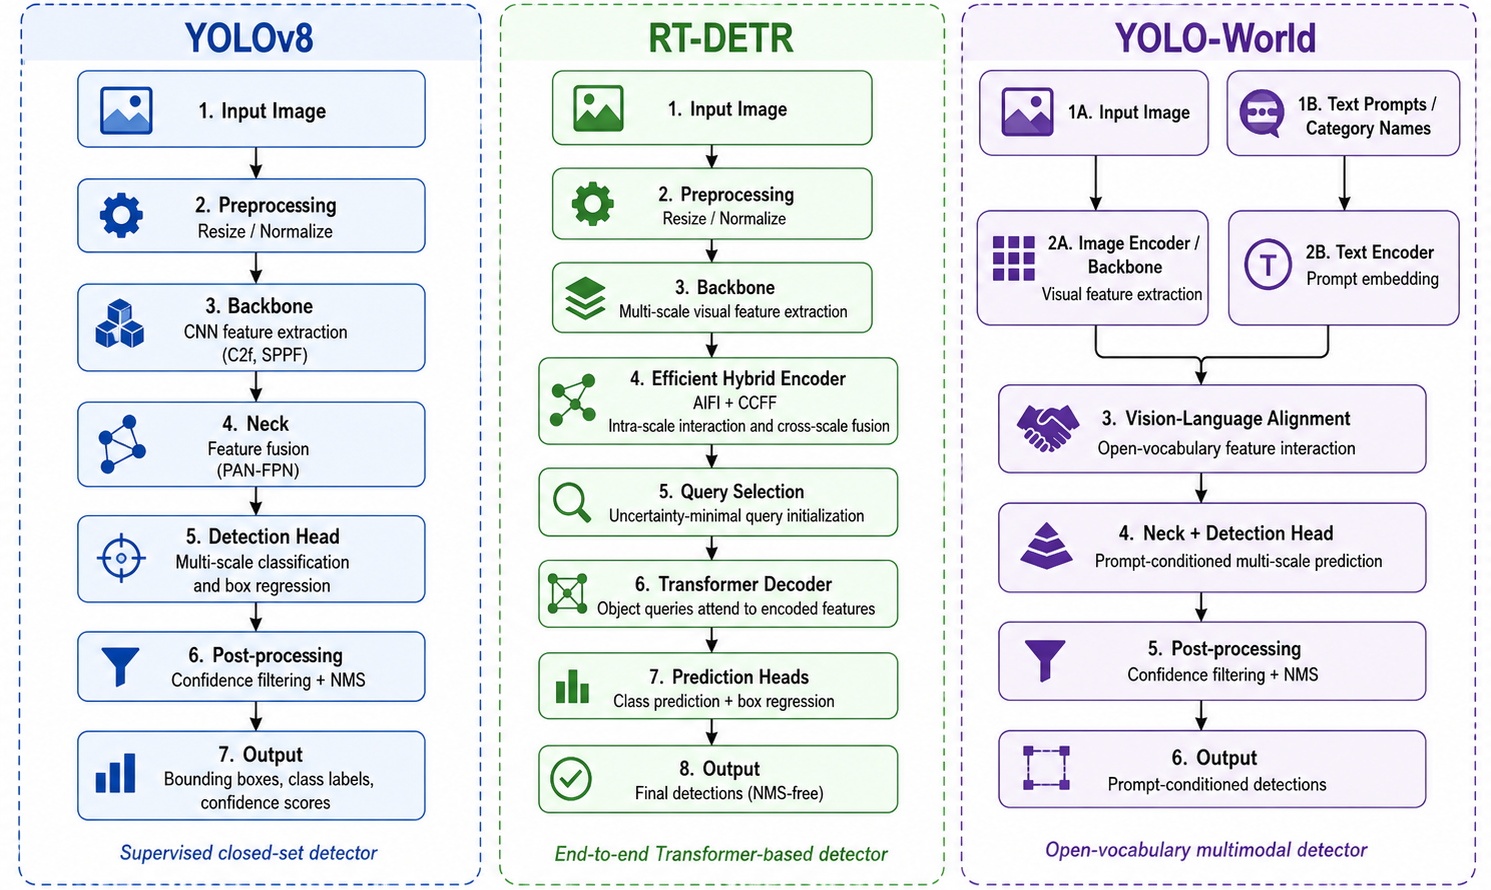
\includegraphics[width=\columnwidth]{model_flowchart.png}
    \caption{The modelling process for the three detectors. YOLOv8 and RT-DETR are trained on each dataset, and YOLO-World is evaluated in a zero-shot prompt sweep and then fine-tuned.}
    \label{fig:model_flowchart}
\end{figure}

The difference that matters for this study is the source of the label space. YOLOv8 predicts boxes and class confidence in a single forward pass and removes duplicates with non-maximum suppression \cite{yolov8}. RT-DETR uses object queries and bipartite matching, which enforces a one-to-one assignment so that duplicate suppression is not required \cite{carion2020detr,zhao2024rtdetr}. For both, the label space is fixed during training. YOLO-World instead scores candidate regions against text embeddings with a contrastive head \cite{cheng2024yoloworld}, so its label space is supplied at inference time as text. YOLO-World is adopted over GLIP because it keeps prompt-based detection inside the same training and evaluation pipeline as the other two models.

\subsection{Datasets}
\label{sec:datasets}

Two evaluation datasets are used, and a third is used only as a reference check. The container dataset is a public port container dataset with a single annotated class, the container number, comprising 1001 images \cite{containerdataset2024}. It is used as an open proxy for the industrial setting, because the original private dataset is not available for release and reproducibility requires a dataset that a third party can obtain. The images are captured during routine gate and handling operations, and they include daytime and night captures, oblique and upward camera angles, surface rust and paint damage, overexposed and backlit frames, and container bodies dominated by red and brown liveries with white printed codes. The printed code appears in both the horizontal and vertical ISO 6346 layouts. The single target region is small, occupying about two percent of the image on average, as reported below.

The ICDAR 2015 dataset provides incidental scene text captured under difficult conditions including blur, low resolution, arbitrary orientation, and irregular layout, and its ground truth is annotated with quadrilateral polygons rather than axis-aligned boxes \cite{icdar2015}. It is included because it is a harder and denser text detection task than the container dataset, and it therefore supplies the difficulty contrast that the near-saturated container data does not.

COCO 2017 provides general object detection with 80 common categories \cite{coco}. It is not part of the training comparison. It is used only to check that the evaluation pipeline is correct, by confirming that the pretrained detectors reproduce their published accuracy, and to observe open-vocabulary behaviour on common categories.

Table~\ref{tab:dataset} characterises the two evaluation datasets. The container dataset has one box per image and a uniform image size. ICDAR 2015 is dense, with about four text instances per image, and its text regions are much smaller relative to the image. The illegible regions marked as ignore in ICDAR 2015 were dropped, which removed 7418 training and 3153 test regions.

\begin{table*}[tb]
\centering
\caption{Dataset characterisation for the two evaluation datasets. Box area is the fraction of the image area covered by a box. One container training image contains no annotated box, giving 701 images and 700 boxes.}
\label{tab:dataset}
\begin{tabular}{llrrrrr}
\toprule
Dataset & Split & Images & Boxes & Boxes/img & Box area p50 & Box area p95 \\
\midrule
Container & train & 701 & 700 & 1.00 & 0.0193 & 0.0375 \\
Container & valid & 200 & 200 & 1.00 & 0.0193 & 0.0403 \\
Container & test  & 100 & 100 & 1.00 & 0.0195 & 0.0440 \\
ICDAR 2015 & train & 1000 & 4468 & 4.47 & 0.0022 & 0.0166 \\
ICDAR 2015 & test  & 500 & 2077 & 4.15 & 0.0024 & 0.0209 \\
\bottomrule
\end{tabular}
\end{table*}

\subsection{Data Preprocessing}
\label{sec:preproc}

The datasets were reorganised into a unified structure. The ICDAR 2015 text polygons were converted into axis-aligned bounding boxes so that the label format is identical across the three models, and the effect of this conversion on the scores is discussed in Sect.~\ref{sec:limitations}. The container dataset was re-split from a pooled list of the 1001 source images into 70/20/10 train, validation, and test subsets with a fixed random seed. A leak check confirmed 1001 unique source images and no image shared between splits.

\subsection{Implementation and Evaluation Protocol}
\label{sec:protocol}

All three models were run through the Ultralytics implementations so that data loading, augmentation defaults, and metric computation were shared. YOLOv8 and RT-DETR were trained on each evaluation dataset. YOLO-World was first evaluated in zero-shot mode across several prompts and then fine-tuned on each dataset and evaluated again. Table~\ref{tab:config} lists the configuration in full so that the experiments can be replicated.

\begin{table*}[tb]
\centering
\caption{Training and evaluation configuration. The same settings were used for all datasets unless noted.}
\label{tab:config}
\begin{tabular}{ll}
\toprule
Setting & Value \\
\midrule
Model variants & \texttt{yolov8s.pt}, \texttt{rtdetr-l.pt}, \texttt{yolov8s-worldv2.pt} \\
Training & image size 640, 100 epochs, batch 16 (RT-DETR 8) \\
Optimizer & auto, lr0 0.01, lrf 0.01, patience 50, seed 0 \\
Split (container) & 70/20/10 train/val/test, seed 0; reported on held-out test \\
Software & Ultralytics 8.3.40, PyTorch 2.10.0+cu128, CUDA 12.8, Python 3.12.13 \\
Hardware & NVIDIA Tesla T4 \\
\bottomrule
\end{tabular}
\end{table*}

All accuracy results for the container and ICDAR 2015 datasets are reported on the held-out test split, not the validation split. The zero-shot prompts were varied to test whether the outcome depends on wording: eight prompt formulations for the container dataset, four for ICDAR 2015, and the 80 standard category names for COCO.

The evaluation metrics are precision, recall, mAP50, and mAP50-95. The primary metric is mAP50-95, which averages average precision over intersection-over-union thresholds from 0.50 to 0.95 and is the stricter of the two. For the supervised models the checkpoint with the highest validation mAP50-95 is used for test evaluation, and for the zero-shot setting the best result across the prompt sweep is reported alongside the sweep. The complete code, prompt sets, configuration files, and the aggregated result CSVs are released at \url{https://github.com/looxinyiing/comparative-study-cnn-transformer-openvocab-container-scene-text-detection}.

\section{Results}

Table~\ref{tab:main} reports the accuracy of the three models on the container and ICDAR 2015 test splits, together with the COCO reference block. Inference cost is reported separately in Table~\ref{tab:latency}. The results support three observations, which correspond to the three research questions.

\begin{table*}[tb]
\centering
\caption{Detection accuracy. Container and ICDAR 2015 are reported on the held-out test split. COCO 2017 is a reference check on the pretrained models and is not part of the training comparison. The zero-shot row reports the best result across the prompt sweep.}
\label{tab:main}
\begin{tabular}{llcccc}
\toprule
Dataset & Model / Setting & Precision & Recall & mAP50 & mAP50-95 \\
\midrule
Container & YOLOv8 supervised & 0.9898 & \textbf{1.0000} & \textbf{0.9950} & 0.9079 \\
Container & RT-DETR supervised & \textbf{1.0000} & 0.9989 & \textbf{0.9950} & 0.9046 \\
Container & YOLO-World fine-tuned & 0.9974 & 0.9900 & 0.9948 & \textbf{0.9181} \\
Container & YOLO-World zero-shot (best) & 0.0156 & 0.0400 & 0.0082 & 0.0033 \\
\midrule
ICDAR 2015 & YOLOv8 supervised & 0.7294 & 0.6737 & 0.7301 & 0.4352 \\
ICDAR 2015 & RT-DETR supervised & 0.7064 & \textbf{0.6842} & \textbf{0.7355} & \textbf{0.4526} \\
ICDAR 2015 & YOLO-World fine-tuned & \textbf{0.7443} & 0.6348 & 0.7245 & 0.4214 \\
ICDAR 2015 & YOLO-World zero-shot (best) & 0.0083 & 0.0193 & 0.0052 & 0.0018 \\
\midrule
COCO 2017 & YOLOv8 pretrained & 0.6841 & 0.5620 & 0.6132 & 0.4484 \\
COCO 2017 & RT-DETR pretrained & 0.7432 & 0.6545 & 0.7021 & 0.5214 \\
COCO 2017 & YOLO-World zero-shot (80 cats) & 0.6006 & 0.4859 & 0.5170 & 0.3748 \\
\bottomrule
\end{tabular}
\end{table*}

\subsection{Supervised Comparison and the Pipeline Check}

On the container test split, all three supervised or fine-tuned models perform similarly, with fine-tuned YOLO-World highest at 0.9181, YOLOv8 at 0.9079, and RT-DETR at 0.9046, and all three reaching mAP50 near 0.995. The task is therefore close to saturated for a supervised model, which is consistent with the single class and the uniform capture format, so the container dataset tests robustness to capture conditions rather than task difficulty.

On ICDAR 2015, the same models reach much lower scores, between 0.42 and 0.45 mAP50-95. RT-DETR is the most accurate at 0.4526, ahead of YOLOv8 at 0.4352 and fine-tuned YOLO-World at 0.4214. This gap between the container and ICDAR results, about 0.91 against about 0.44, is the difficulty contrast referred to in Sect.~\ref{sec:datasets}. Part of the low ICDAR value is a property of the evaluation, as discussed in Sect.~\ref{sec:limitations}, but the ranking among the three models is meaningful because they use identical labels.

The COCO block is a check on the pipeline rather than a result of interest. The pretrained YOLOv8 reaches 0.4484 mAP50-95 against a published value of about 0.449, and the pretrained RT-DETR reaches 0.5214 against about 0.530, both within 0.03 of the published figures. This indicates that the evaluation pipeline is correct and that the container and ICDAR numbers are not a measurement artefact. Zero-shot YOLO-World reaches 0.3748 on COCO with the 80 category names, so the model is competitive when the target categories are common and well represented in pre-training data.

\subsection{Zero-Shot Failure and Prompt Sensitivity}

The clearest result is the failure of the zero-shot open-vocabulary detector on both text datasets. Zero-shot YOLO-World reaches only 0.0033 mAP50-95 on the container test split and 0.0018 on ICDAR 2015. Table~\ref{tab:prompts} reports the full prompt sweep: eight container prompts (from the plain class name to descriptive phrases such as white text on shipping container) and four ICDAR prompts, with the best reaching 0.0033 and 0.0018 respectively and every prompt staying below 0.10. The failure is therefore robust to how the target is described in language.

\begin{table}[tb]
\centering
\caption{Zero-shot prompt sweep for YOLO-World on the test splits. No fine-tuning. Every prompt on both datasets stays below 0.10 mAP50-95.}
\label{tab:prompts}
\footnotesize
\setlength{\tabcolsep}{4pt}
\begin{tabular}{cl>{\raggedright\arraybackslash}p{3.4cm}cc}
\toprule
Dataset & \# & Prompt & mAP50 & mAP50-95 \\
\midrule
\multirow{8}{*}{Container}
 & 1 & container-number & 0.0000 & 0.0000 \\
 & 2 & container number & 0.0000 & 0.0000 \\
 & 3 & text & 0.0023 & 0.0005 \\
 & 4 & serial number & 0.0000 & 0.0000 \\
 & 5 & white text on shipping container & 0.0012 & 0.0008 \\
 & 6 & identification code on cargo container & 0.0000 & 0.0000 \\
 & 7 & letters and numbers & \textbf{0.0082} & \textbf{0.0033} \\
 & 8 & printed text & 0.0058 & 0.0012 \\
\midrule
\multirow{4}{*}{ICDAR 2015}
 & 1 & text & 0.0012 & 0.0002 \\
 & 2 & word & 0.0029 & 0.0004 \\
 & 3 & scene text & \textbf{0.0052} & \textbf{0.0018} \\
 & 4 & printed text & 0.0000 & 0.0000 \\
\bottomrule
\end{tabular}
\end{table}

Fig.~\ref{fig:container_qual} compares supervised YOLOv8 and zero-shot YOLO-World on the same two container test images. YOLOv8 localises the code region in both the horizontal and the vertical layout, whereas zero-shot YOLO-World returns almost no boxes above the confidence threshold. The same empty output occurred on ICDAR 2015, where the supervised detectors localise scene text regions.

\begin{figure}[tb]
    \centering
    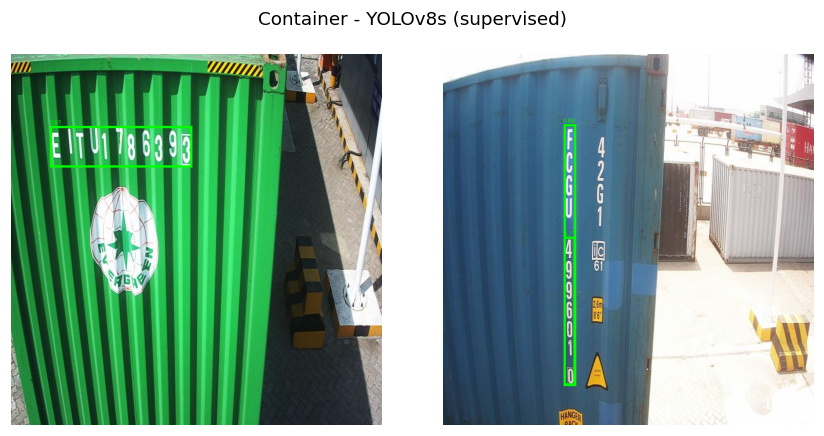
\includegraphics[width=\columnwidth]{fig_container_yolov8s.png}\\[2pt]
    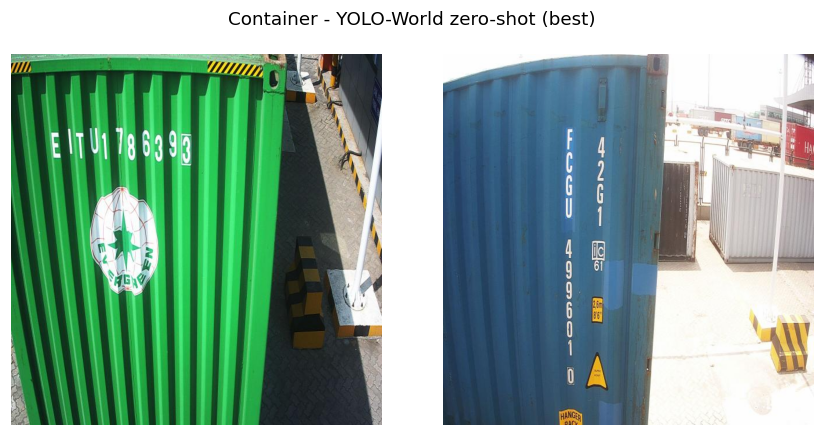
\includegraphics[width=\columnwidth]{fig_container_world_zs.png}
    \caption{Qualitative comparison on two container test images. Top: supervised YOLOv8 localises the container-number region (green boxes) in both the horizontal and the vertical ISO 6346 layout. Bottom: zero-shot YOLO-World with its best prompt returns almost no boxes on the same images (0.0033 mAP50-95 against about 0.91 for the supervised detectors, Table~\ref{tab:main}).}
    \label{fig:container_qual}
\end{figure}

\subsection{Effect of Fine-Tuning}

Fine-tuning recovers the gap. YOLO-World mAP50-95 increases from 0.0033 to 0.9181 on the container dataset and from 0.0018 to 0.4214 on ICDAR 2015, while on COCO the zero-shot value of 0.3748 needs no such recovery. The improvement is largest where the target is most domain-specific, so YOLO-World has useful adaptation capacity but requires target-domain supervision on these text categories.

\subsection{Inference Cost}

Table~\ref{tab:latency} reports inference latency and peak GPU memory at batch size one. YOLOv8 is fastest at 8.94 ms. YOLO-World runs at a similar speed, 9.28 ms, but carries the largest memory footprint at 725.4 MB because the text encoder is resident. RT-DETR is the slowest at 46.31 ms, about five times slower than YOLOv8. Parameter counts are not reported since the YOLO-World count includes the text encoder and is not comparable to the other two. Measurements use the pretrained architectures, as discussed in Sect.~\ref{sec:limitations}.

\begin{table}[tb]
\centering
\caption{Inference latency and peak GPU memory, measured on a Tesla T4 at image size 640 and batch size 1. Lower latency and lower memory are better.}
\label{tab:latency}
\begin{tabular}{lccc}
\toprule
Model & Inference (ms) & FPS & Peak GPU memory (MB) \\
\midrule
YOLOv8 & \textbf{8.94} & \textbf{111.9} & \textbf{102.8} \\
RT-DETR & 46.31 & 21.6 & 289.0 \\
YOLO-World & 9.28 & 107.7 & 725.4 \\
\bottomrule
\end{tabular}
\end{table}

\section{Discussion}

\subsection{Interpretation of the Model Paradigms}

No single paradigm wins on both text tasks and inference cost. RT-DETR leads on the harder ICDAR 2015 task, consistent with the value of global attention and end-to-end set prediction when text is dense, but at about five times the inference time of YOLOv8. On the container task the three models are too close to rank with confidence. For a real-time gate system the latency of RT-DETR may outweigh a small accuracy gain, so the choice between a CNN-based and a Transformer-based detector is a trade-off between accuracy and speed.

\subsection{Why Zero-Shot Open-Vocabulary Detection Fails Here}

The zero-shot failure is consistent across datasets and prompts, and it has a plausible explanation. Terms such as text, container number, and scene text describe functional or semantic regions rather than visually distinct natural objects. A container number is not any text region, but a specific printed identifier in a specific location and layout, and this distinction depends on annotation conventions that the category name does not carry. The targets are also small, occupying about two percent of the image for the container code and less for ICDAR text, whereas open-vocabulary detectors are trained mainly on object-level concepts at larger scales. Both factors push the target outside the pre-training distribution. Fine-tuning supplies both the category definition and the expected box scale, which is consistent with the size of the observed recovery.

The practical message is that supervised training remains necessary for a fixed operational environment, because open-vocabulary pre-training in the detector evaluated here does not remove the labelling step. For container code detection YOLOv8 and fine-tuned YOLO-World both reach high accuracy, with YOLOv8 the more efficient choice. An open-vocabulary model is worthwhile only where target categories may change after deployment and only with target-domain fine-tuning, at a higher memory cost.

\subsection{Limitations}
\label{sec:limitations}

This study has several limitations, and the following are stated explicitly because they affect how the reported numbers should be read. The container dataset is a single-class public dataset, annotated only with the container number, so a per-class analysis across categories such as container number, type code, and nameplate is out of scope. The original industrial dataset with those categories is not publicly available, which is the reason for the substitution. The container task is also near-saturated for a supervised model, at about 0.91 mAP50-95, and its appearance diversity is limited, with the container bodies dominated by red and brown liveries and the printed codes almost always white. The container results should therefore be read as evidence of robustness to varying capture conditions rather than to varying container appearance, and the difficulty contrast in this study comes from ICDAR 2015. Each model was trained once with a single random seed, so no variance is reported, and small differences between models should not be over-interpreted.

For ICDAR 2015 the polygonal ground truth was converted to axis-aligned boxes. The axis-aligned box enclosing an oriented polygon also encloses background, so the intersection-over-union attainable against a correct prediction is bounded below one. This penalty grows with the stricter thresholds averaged in mAP50-95 and applies to every model equally, so the absolute ICDAR values are depressed and should not be compared in magnitude with the container results or with polygon-based results in the literature. The ranking among the three models is unaffected. Inference latency and memory were measured on the pretrained architectures rather than the fine-tuned checkpoints, which were not retained; both depend on architecture and input size rather than learned weights, so the measurements remain valid at the architecture level.

The study evaluates detection only and does not measure downstream character recognition, which is a necessary component of a complete industrial reading system. The open-vocabulary paradigm is also represented by YOLO-World alone, so the results should be read as an evaluation of a YOLO-style open-vocabulary detector rather than of vision-language detectors in general. Future work should therefore extend this study with a multi-class industrial dataset, multi-seed training with variance estimates, polygon-aware scene-text evaluation, end-to-end recognition, and further open-vocabulary detectors such as GLIP or Grounding DINO.

\section{Conclusion}

This study compared CNN-based, Transformer-based, and open-vocabulary detectors for cargo container and scene text detection under a single evaluation protocol, on a public container dataset and on ICDAR 2015, with COCO 2017 as a pipeline check. The three research questions can be answered as follows.

On RQ1, the CNN-based and Transformer-based detectors are close on the container task, within 0.004 mAP50-95, and separated on the harder scene text task, where RT-DETR leads at 0.4526 against YOLOv8 at 0.4352. When inference cost is included, YOLOv8 is preferable where its small accuracy deficit is acceptable, because RT-DETR is about five times slower.

On RQ2, the open-vocabulary detector could not locate container or scene text targets from prompts alone. Zero-shot YOLO-World reached 0.0033 mAP50-95 on the container test split and 0.0018 on ICDAR 2015, and this held across all eight container and four scene-text prompts, so it is not sensitive to prompt wording. The same model reached 0.3748 on COCO, which shows the failure is specific to the domain rather than to the model. The answer to RQ2 is negative for the prompts evaluated here.

On RQ3, fine-tuning closed the gap, raising container mAP50-95 from 0.0033 to 0.9181 and ICDAR 2015 from 0.0018 to 0.4214, while COCO needed no such recovery. The size of the improvement scales with how domain-specific the target is, which is consistent with fine-tuning supplying the annotation conventions and the box scale that the prompt does not carry.

Taken together, the open-vocabulary detector evaluated here does not remove the labelling step for container or scene text detection. Target-domain supervision remains necessary, and among the supervised options the choice depends on both accuracy and inference cost. These conclusions apply to the datasets and prompts evaluated here, and the stricter evaluations in Sect.~\ref{sec:limitations} are needed before they can be generalised further.

\begin{thebibliography}{00}

\bibitem{allread2024maritime} AllRead MLT, ``OCR for maritime terminals and gate automation,'' 2024. [Online]. Available: \url{https://www.allread.ai/en/ocr-applications/maritime-terminal-ocr/}

\bibitem{scanbot2024iso6346} Scanbot SDK, ``Container OCR: Scanning ISO 6346 codes,'' 2024. [Online]. Available: \url{https://scanbot.io/blog/container-ocr-for-iso-6346-codes/}

\bibitem{santos2025container} J. Santos, D. Canedo, and A. J. R. Neves, ``Automating code recognition for cargo containers,'' \textit{Electronics}, vol. 14, no. 22, p. 4437, 2025.

\bibitem{redmon2016yolo} J. Redmon, S. Divvala, R. Girshick, and A. Farhadi, ``You only look once: Unified, real-time object detection,'' in \textit{Proc. IEEE Conf. Comput. Vis. Pattern Recognit. (CVPR)}, 2016, pp. 779--788.

\bibitem{redmon2018yolov3} J. Redmon and A. Farhadi, ``YOLOv3: An incremental improvement,'' \textit{arXiv preprint arXiv:1804.02767}, 2018.

\bibitem{yolov8} Ultralytics, ``YOLOv8,'' 2023. [Online]. Available: \url{https://github.com/ultralytics/ultralytics}

\bibitem{carion2020detr} N. Carion, F. Massa, G. Synnaeve, N. Usunier, A. Kirillov, and S. Zagoruyko, ``End-to-end object detection with transformers,'' in \textit{Proc. Eur. Conf. Comput. Vis. (ECCV)}, 2020.

\bibitem{zhao2024rtdetr} Y. Zhao, W. Lv, S. Xu, J. Wei, G. Wang, Q. Dang, Y. Liu, and J. Chen, ``DETRs beat YOLOs on real-time object detection,'' in \textit{Proc. IEEE/CVF Conf. Comput. Vis. Pattern Recognit. (CVPR)}, 2024.

\bibitem{li2022glip} L. H. Li, P. Zhang, H. Zhang, J. Yang, C. Li, Y. Zhong, L. Wang, L. Yuan, L. Zhang, J.-N. Hwang, K.-W. Chang, and J. Gao, ``Grounded language-image pre-training,'' in \textit{Proc. IEEE/CVF Conf. Comput. Vis. Pattern Recognit. (CVPR)}, 2022.

\bibitem{gu2022vild} X. Gu, T.-Y. Lin, W. Kuo, and Y. Cui, ``Open-vocabulary object detection via vision and language knowledge distillation,'' in \textit{Proc. Int. Conf. Learn. Represent. (ICLR)}, 2022.

\bibitem{cheng2024yoloworld} T. Cheng, L. Song, Y. Ge, W. Liu, X. Wang, and Y. Shan, ``YOLO-World: Real-time open-vocabulary object detection,'' \textit{arXiv preprint arXiv:2401.17270}, 2024.

\bibitem{zhou2017east} X. Zhou, C. Yao, H. Wen, Y. Wang, S. Zhou, W. He, and J. Liang, ``EAST: An efficient and accurate scene text detector,'' in \textit{Proc. IEEE Conf. Comput. Vis. Pattern Recognit. (CVPR)}, 2017, pp. 5551--5560.

\bibitem{long2018textsnake} S. Long, J. Ruan, W. Zhang, X. He, W. Wu, and C. Yao, ``TextSnake: A flexible representation for detecting text of arbitrary shapes,'' in \textit{Proc. Eur. Conf. Comput. Vis. (ECCV)}, 2018.

\bibitem{liao2020dbnet} M. Liao, Z. Wan, C. Yao, K. Chen, and X. Bai, ``Real-time scene text detection with differentiable binarization,'' in \textit{Proc. AAAI Conf. Artif. Intell.}, 2020.

\bibitem{liu2020abcnet} Y. Liu, H. Chen, C. Shen, T. He, L. Jin, and L. Wang, ``ABCNet: Real-time scene text spotting with adaptive Bezier-curve network,'' in \textit{Proc. IEEE/CVF Conf. Comput. Vis. Pattern Recognit. (CVPR)}, 2020, pp. 9809--9818.

\bibitem{containerdataset2024} Roboflow Universe contributor, ``Container number detection dataset, version 3,'' Roboflow Universe, 2024, single class \texttt{container-number}, 1001 images, licensed CC BY 4.0.

\bibitem{icdar2015} D. Karatzas \textit{et al.}, ``ICDAR 2015 competition on robust reading,'' in \textit{Proc. Int. Conf. Document Anal. Recognit. (ICDAR)}, 2015.

\bibitem{coco} T.-Y. Lin, M. Maire, S. Belongie, J. Hays, P. Perona, D. Ramanan, P. Doll\'ar, and C. L. Zitnick, ``Microsoft COCO: Common objects in context,'' in \textit{Proc. Eur. Conf. Comput. Vis. (ECCV)}, 2014.

\end{thebibliography}

\end{document}
